\documentclass[a4paper,9pt,twocolumn,twoside,]{pinp}

%% Some pieces required from the pandoc template
\providecommand{\tightlist}{%
  \setlength{\itemsep}{0pt}\setlength{\parskip}{0pt}}

% Use the lineno option to display guide line numbers if required.
% Note that the use of elements such as single-column equations
% may affect the guide line number alignment.

\usepackage[T1]{fontenc}
\usepackage[utf8]{inputenc}

% pinp change: the geometry package layout settings need to be set here, not in pinp.cls
\geometry{layoutsize={0.95588\paperwidth,0.98864\paperheight},%
  layouthoffset=0.02206\paperwidth, layoutvoffset=0.00568\paperheight}

\definecolor{pinpblue}{HTML}{185FAF}  % imagecolorpicker on blue for new R logo
\definecolor{pnasbluetext}{RGB}{101,0,0} %



\title{Executive Summary Report}

\author[]{R10-08}


\setcounter{secnumdepth}{0}

% Please give the surname of the lead author for the running footer
\leadauthor{R10-08}

% Keywords are not mandatory, but authors are strongly encouraged to provide them. If provided, please include two to five keywords, separated by the pipe symbol, e.g:
 

\begin{abstract}
Your abstract will be typeset here, and used by default a visually
distinctive font. An abstract should explain to the general reader the
major contributions of the article.
\end{abstract}

\dates{This version was compiled on \today} 

% initially we use doi so keep for backwards compatibility
% new name is doi_footer
\doifooter{\url{https://github.sydney.edu.au/kvoo2843/R10-08.git}}

\pinpfootercontents{Executive Summary Report - Wine Quality}

\begin{document}

% Optional adjustment to line up main text (after abstract) of first page with line numbers, when using both lineno and twocolumn options.
% You should only change this length when you've finalised the article contents.
\verticaladjustment{-2pt}

\maketitle
\thispagestyle{firststyle}
\ifthenelse{\boolean{shortarticle}}{\ifthenelse{\boolean{singlecolumn}}{\abscontentformatted}{\abscontent}}{}

% If your first paragraph (i.e. with the \dropcap) contains a list environment (quote, quotation, theorem, definition, enumerate, itemize...), the line after the list may have some extra indentation. If this is the case, add \parshape=0 to the end of the list environment.


\subsection{Introduction}\label{introduction}

Using the dataset provided, we tried to create a suitable model that
determines the predictive power of the input variables. In our case, our
goal is to create a model that can be used to predict the quality of red
wine, based on the predictor variables selected, based on both a forward
and backwards stepwise variable selection process, and then choosing the
more suitable model, preferably the one with less variables. We will
then discuss the limitations, and potential improvements to our model.

\subsection{Dataset Description}\label{dataset-description}

This dataset is from the UCI Machine Learning Repository and contains
variables relating to the makeup of Portuguese ``Vinho Verde'' wines.
White wine and red wine is divided into two separate datasets. We chose
to only build a model on the red wine dataset, due to the specifications
asking for only one dataset to be analysed. There are a total of 1597
observations in this red wine dataset. This dataset in its current form
was originally intended to model wine preferences via machine learning.

Variables consist of both input and output variables. Input variables
include:

\begin{itemize}
\tightlist
\item
  \textbf{Fixed Acidity}: Acidity that naturally occurs in the grapes.
\item
  \textbf{Volitile Acidity}: Acidity produced from bacteria. High
  volatile acidity is known to be a sign of spoilage.
\item
  \textbf{Citric Acid}: Both added and naturally occuring. Most of it is
  fermented away in fermentation.
\item
  \textbf{Residual Sugar}: Natural sugars from grapes that did not
  ferment in the wine making process.
\item
  \textbf{Chlorides}: Measurement of salt content
\item
  \textbf{Free Sulfur Dioxide}: Portion free in the wine
\item
  \textbf{Total Sulfur Dioxide}: Portion bonded to other chemicals in
  the wine
\item
  \textbf{Density}: Mass per volume
\item
  \textbf{PH}: Measurement of the wine's acidity
\item
  \textbf{Sulphates}: Additive from the wine making process to allow
  freshness
\item
  \textbf{Alcohol}: Measurement of the overall alcohol proportion in the
  sample \newline(Winemaker's Academy, 2013)
\end{itemize}

The output variable is a quality rating out of 10. This is a discrete
set between 1 and 10 inclusive. Most quality scores were around 5 or 6
out of 10, with an interquartile range of 1, as shown in fig 1. A total
of 82\% of all observations received these scores. The top quality score
was 8, with the bottom quality score 3, providing a range of 5. But
there were much fewer observations the further away from Q1 and Q3 the
quality was. This can be seen in figure 1.

\begin{figure}

{\centering 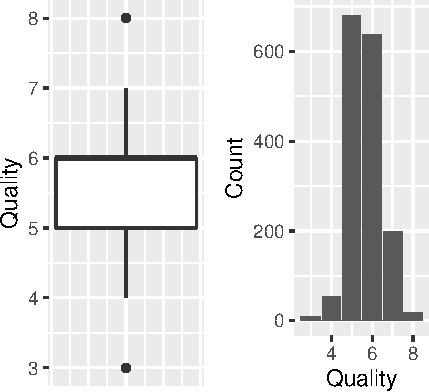
\includegraphics{Executive_Summary_files/figure-latex/figex-1} 

}

\caption{Boxplot and Histogram of Quality scores}\label{fig:figex}
\end{figure}

\subsection{Analysis}\label{analysis}

We initially began work on our model selection by creating two different
models using 2 different approaches. The first model created was a
`Stepwise Backward' model, where we started out with an initial full
model, and reduced the size of the model by dropping variables that were
insignificant at the 5\% level of significance. We dropped the variables
in sequence, based on the largest p-values.

We eventually encountered a variable \emph{residual sugar}, that had a
p-value of around \textbf{0.13}. We decided to also drop the variable,
as although it is significant at the 5\% level of significance, it would
become insignificant at the 1\% level of significance. We then created
another Forward model using AIC, with R. Once we had our 2 models, we
then compared to see which of the 2 would be the more suitable model. We
noticed that the \(R^2\) values were almost identical, and the adjusted
\(R^2\) values were the same between the 2 models
\hyperref[table-1]{(see Table 1)}, and so we selected the model with the
least amount of variables out of the 2 as our model. That being the
Stepwise Backward model \hyperref[table-1]{(see Table 1 (1))}.

\subsubsection{The final model can be defined
as:}\label{the-final-model-can-be-defined-as}

\begin{equation}
  \begin{aligned}
  quality = \beta_{0} + \beta_{1}{x_1} + \beta_{2}{x_2} + \beta_{3}{x_3} + ... + \beta_{7}{x_7} + \beta_{8}{x_8} + \epsilon_i
       \label{eqn:model}
  \end{aligned}
\end{equation}

\begin{itemize}
\tightlist
\item
  \(x_1\) = volatile acidity
\item
  \(x_2\) = density
\item
  \(x_3\) = sulphates
\item
  \(x_4\) = chlorides
\item
  \(x_5\) = total sulfur dioxide
\item
  \(x_6\) = citric acid
\item
  \(x_7\) = free sulfur dioxide
\item
  \(x_8\) = alcohol
\end{itemize}

Once we had our model, we began to check the regression assumptions for
our selected model. \pagebreak

\subsubsection{Assumption checking}\label{assumption-checking}

\begin{itemize}
\tightlist
\item
  \textbf{Linearity}: Upon observing the residual vs fitted values plot,
  the graph showed elements of linearity as there was no obvious pattern
  shown in the graph, such as a parabolic shape. As such, the normal
  assumption is not violated, and it doesn't appear that we have
  misspecified the model.
\item
  \textbf{Independence}: Based on the nature of the dataset, we made the
  assumption that each sampling of wine does not affect the other wine
  samples. We also assumed the wines were choosen at random. That would
  mean all errors are independent of each other. Furthermore, the
  dataset we are working with does not deal with time series data,
  reducing the likelihood of the independence assumption being violated.
  As such, the independence assumption is at least approximately
  satisfied.\\
\item
  \textbf{Homoskedasticity}: Based on the scatter plot, the residuals
  for each fitted value appears mostly equal in spread, apart for some
  outliers. So, the constant error variance assumption is met.
\item
  \textbf{Normality}: In the QQ plot, it is very obvious that the points
  are reasonably close to the diagonal line. The bottom left end points
  are not quite on the line, but is not severe enough to influence the
  results. As such, the normality assumption is at least approximately
  satisfied.
\end{itemize}

\begin{figure}

{\centering 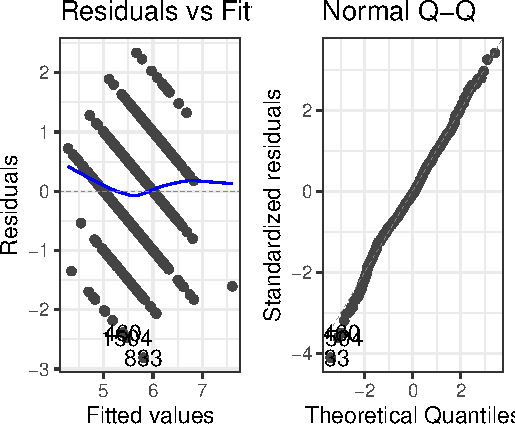
\includegraphics{Executive_Summary_files/figure-latex/unnamed-chunk-3-1} 

}

\caption{Checking linear assumptions for the backwards stepwise model.}\label{fig:unnamed-chunk-3}
\end{figure}

\subsection{Results}\label{results}

Looking at the \(R^2\) value from the summary output
\hyperref[table-1]{(see Table 1)}, 28\% (see discussion for details) of
the variablity of the wine quality is explained by the regression on the
8 predictor variables in our model.

Using the final model, we are able to estimate the average quality of
wine or the quality of a single sample of wine with specific properties
(predictor variables). By using a confidence interval to estimate the
average quality, and prediction interval for predicting a single sample
of wine. A thing to note is that the full model is not particularly good
at making predictions on exceptionally good or bad wines, as the dataset
is very unbalanced. Most (50\%) of the quality values are either 5 or 6.

Below is a quick demonstration of a prediction interval prediction using
the first entry from the dataset.

\begin{ShadedResult}
\begin{verbatim}
#  Observations: 1
#  Variables: 8
#  $ volatile_acidity     <dbl> 0.7
#  $ citric_acid          <dbl> 0
#  $ chlorides            <dbl> 0.076
#  $ free_sulfur_dioxide  <dbl> 11
#  $ total_sulfur_dioxide <dbl> 34
#  $ density              <dbl> 0.9978
#  $ alcohol              <dbl> 94
#  $ quality              <dbl> 5
\end{verbatim}
\end{ShadedResult}\begin{ShadedResult}
\begin{verbatim}
#         fit      lwr      upr
#  1 5.176034 3.829332 6.522736
\end{verbatim}
\end{ShadedResult}

The predicted quality was about 5.18, which was roughly the same as the
actual quality value in the dataset which was 5.

\subsection{Discussion \& Conclusion}\label{discussion-conclusion}

When we first plotted our residuals vs fitted values and qq-plot graphs,
we then noticed the unorthodox shape of the residual vs fitted graph. We
then realised that it was due to the dependent variable, quality, being
discrete values. We made an attempt to log the dependent variable in an
attempt to improve the shape of the graph, but there were no noticable
changes to the model, and decided to leave the values discrete.

It was noticed that the \(R^2\) values were low, at approximately 28\%.
This was mostly a result of the dataset being very unbalanced, as
mentioned before in the dataset description, where 82\% of the values
were either 5 of 6.

In order to improve the results, the model was reduced further by
dropping the variable \emph{alcohol}. Although significant even at the
1\% level of significance with a p-value of about 0.025, it was by far
the largest p-value amongst the other values. However, this did not
improve the overall \(R^2\) value, and the changes that occured were
neglible \hyperref[table-2]{(see Table 2)}. As such, we decided to stick
with our final model that is shown \hyperref[eqn:model]{above}.

To try to improve the equal variance assumption, logging the dependant
variable was tested. This was also attempted with the independant
variables. Despite this, there was no improvement in the overall
variance of the model. The weakness of the assumptions may have effected
the \(R^2\) value of the model.

For this model, root mean square error was found to be 0.68. Accounting
for outliers, the mean absolute error was calculated as 0.53, a stronger
measurement for this dataset due to the large cluster of quality scores
around 5 and 6. In contrast, the null model returned a root mean square
error of 0.81 and a mean absolute error of 0.68, which was lower than
the values for the full model. Further testing of out of sample
performance could have been conducted by selecting a proportion of the
dataset to be used as training data, as well as cross validation. This
will be conduced in the future.

Predictions of quality were on the continous scale, but real values in
the dataset were discrete in the series of integers \([1:10]\). This was
ignored for the purposes of this report.

One improvement that could have been made in our analysis, was to
perform formal tests to see if the coefficient for each variable we were
going to drop were significant. By first defining a model with the
relevant parameters, and then forming formal hypothesis and assumptions,
do the relevant assumption checks, find the test statistic, and
p-values, come to a conclusion on whether or not to drop the
variable(s). We did not do this, due to time constraints, and would have
been too labour intensive, and a bit too much work for our purpose.

Overall, there was success in predicting wine quality based on the
dataset's independant variables.

Another improvement, or at least a change we could have made, was to
instead create a model that helps predict good or bad wine. As our model
is only relatively accurate for ``normal'' quality wine.

\pagebreak

\subsection{References}\label{references}

\begin{itemize}
\tightlist
\item
  Understanding Wine Acidity. (2018, June 25). Retrieved from
  \url{http://winemakersacademy.com/understanding-wine-acidity/}.
\item
  P. Cortez, A. Cerdeira, F. Almeida, T. Matos and J. Reis. Modeling
  wine preferences by data mining from physicochemical properties. In
  Decision Support Systems, Elsevier, 47(4):547-553, 2009.
\end{itemize}

\subsection{Appendix}\label{appendix}

\subsubsection{Table 1}\label{table-1}

\begin{itemize}
\item
  \begin{enumerate}
  \def\labelenumi{(\arabic{enumi})}
  \tightlist
  \item
    = Stepwise Backward Model.
  \end{enumerate}
\item
  \begin{enumerate}
  \def\labelenumi{(\arabic{enumi})}
  \setcounter{enumi}{1}
  \tightlist
  \item
    = AIC Forward Model.
  \end{enumerate}
\end{itemize}

\begin{table}[!htbp] \centering 
  \caption{Regression Results} 
  \label{} 
\begin{tabular}{@{\extracolsep{5pt}}lcc} 
\\[-1.8ex]\hline 
\hline \\[-1.8ex] 
 & \multicolumn{2}{c}{\textit{Dependent variable:}} \\ 
\cline{2-3} 
\\[-1.8ex] & \multicolumn{2}{c}{quality} \\ 
\\[-1.8ex] & (1) & (2)\\ 
\hline \\[-1.8ex] 
 volatile\_acidity & $-$0.909$^{***}$ & $-$0.923$^{***}$ \\ 
  & (0.126) & (0.126) \\ 
  & & \\ 
 citric\_acid & 0.629$^{***}$ & 0.610$^{***}$ \\ 
  & (0.122) & (0.123) \\ 
  & & \\ 
 chlorides & $-$3.288$^{***}$ & $-$3.274$^{***}$ \\ 
  & (0.410) & (0.410) \\ 
  & & \\ 
 free\_sulfur\_dioxide & 0.005$^{***}$ & 0.005$^{***}$ \\ 
  & (0.001) & (0.001) \\ 
  & & \\ 
 total\_sulfur\_dioxide & $-$0.006$^{***}$ & $-$0.006$^{***}$ \\ 
  & (0.001) & (0.001) \\ 
  & & \\ 
 density & $-$86.012$^{***}$ & $-$87.214$^{***}$ \\ 
  & (10.337) & (10.365) \\ 
  & & \\ 
 sulphates & 1.246$^{***}$ & 1.252$^{***}$ \\ 
  & (0.116) & (0.116) \\ 
  & & \\ 
 alcohol & 0.000$^{**}$ & 0.000$^{**}$ \\ 
  & (0.000) & (0.000) \\ 
  & & \\ 
 residual\_sugar &  & 0.001 \\ 
  &  & (0.0004) \\ 
  & & \\ 
 Constant & 91.326$^{***}$ & 92.516$^{***}$ \\ 
  & (10.268) & (10.295) \\ 
  & & \\ 
\hline \\[-1.8ex] 
Observations & 1,597 & 1,597 \\ 
R$^{2}$ & 0.283 & 0.284 \\ 
Adjusted R$^{2}$ & 0.280 & 0.280 \\ 
Residual Std. Error & 0.686 (df = 1588) & 0.685 (df = 1587) \\ 
F Statistic & 78.409$^{***}$ (df = 8; 1588) & 69.999$^{***}$ (df = 9; 1587) \\ 
\hline 
\hline \\[-1.8ex] 
\textit{Note:}  & \multicolumn{2}{r}{$^{*}$p$<$0.1; $^{**}$p$<$0.05; $^{***}$p$<$0.01} \\ 
\end{tabular} 
\end{table}

\subsubsection{Table 2}\label{table-2}

\begin{itemize}
\item
  \begin{enumerate}
  \def\labelenumi{(\arabic{enumi})}
  \tightlist
  \item
    = Backward Model with alcohol.
  \end{enumerate}
\item
  \begin{enumerate}
  \def\labelenumi{(\arabic{enumi})}
  \setcounter{enumi}{1}
  \tightlist
  \item
    = Backward Model without alcohol.
  \end{enumerate}
\end{itemize}

\begin{table}[!htbp] \centering 
  \caption{Stepwise Backward Model comparison} 
  \label{} 
\begin{tabular}{@{\extracolsep{5pt}}lcc} 
\\[-1.8ex]\hline 
\hline \\[-1.8ex] 
 & \multicolumn{2}{c}{\textit{Dependent variable:}} \\ 
\cline{2-3} 
\\[-1.8ex] & \multicolumn{2}{c}{quality} \\ 
\\[-1.8ex] & (1) & (2)\\ 
\hline \\[-1.8ex] 
 volatile\_acidity & $-$0.909$^{***}$ & $-$0.895$^{***}$ \\ 
  & (0.126) & (0.126) \\ 
  & & \\ 
 citric\_acid & 0.629$^{***}$ & 0.633$^{***}$ \\ 
  & (0.122) & (0.122) \\ 
  & & \\ 
 chlorides & $-$3.288$^{***}$ & $-$3.304$^{***}$ \\ 
  & (0.410) & (0.411) \\ 
  & & \\ 
 free\_sulfur\_dioxide & 0.005$^{***}$ & 0.005$^{***}$ \\ 
  & (0.001) & (0.001) \\ 
  & & \\ 
 total\_sulfur\_dioxide & $-$0.006$^{***}$ & $-$0.006$^{***}$ \\ 
  & (0.001) & (0.001) \\ 
  & & \\ 
 density & $-$86.012$^{***}$ & $-$86.030$^{***}$ \\ 
  & (10.337) & (10.350) \\ 
  & & \\ 
 sulphates & 1.246$^{***}$ & 1.249$^{***}$ \\ 
  & (0.116) & (0.116) \\ 
  & & \\ 
 alcohol & 0.000$^{**}$ &  \\ 
  & (0.000) &  \\ 
  & & \\ 
 Constant & 91.326$^{***}$ & 91.335$^{***}$ \\ 
  & (10.268) & (10.281) \\ 
  & & \\ 
\hline \\[-1.8ex] 
Observations & 1,597 & 1,597 \\ 
R$^{2}$ & 0.283 & 0.281 \\ 
Adjusted R$^{2}$ & 0.280 & 0.278 \\ 
Residual Std. Error & 0.686 (df = 1588) & 0.686 (df = 1589) \\ 
F Statistic & 78.409$^{***}$ (df = 8; 1588) & 88.661$^{***}$ (df = 7; 1589) \\ 
\hline 
\hline \\[-1.8ex] 
\textit{Note:}  & \multicolumn{2}{r}{$^{*}$p$<$0.1; $^{**}$p$<$0.05; $^{***}$p$<$0.01} \\ 
\end{tabular} 
\end{table}

%\showmatmethods


\bibliography{pinp}
\bibliographystyle{jss}



\end{document}

